\documentclass{ntuthesis}

\usepackage{times}
\usepackage{verbatim}
\usepackage{color}
\usepackage{url}
\usepackage{graphicx}
\usepackage{array}
\usepackage{fontspec}
\usepackage{hyperref}
\usepackage{commath}
\usepackage{algorithm}
\usepackage{algorithmic}
\usepackage{amsthm}
\usepackage{caption}
\usepackage{amssymb}
\usepackage{amsfonts}
%\usepackage{indentfirst}

% Using the tex-text mapping for ligatures etc.
\defaultfontfeatures{Mapping=tex-text}

% Set the default fonts
\setmainfont{Times New Roman}
\setCJKmainfont{BiauKai}

% Your information goes here
% author: Tz-Huan Huang [http://www.csie.ntu.edu.tw/~tzhuan]

% ----------------------------------------------------------------------------
% "THE CHOCOLATE-WARE LICENSE":
% Tz-Huan Huang wrote this file. As long as you retain this notice you
% can do whatever you want with this stuff. If we meet some day, and you think
% this stuff is worth it, you can buy me a chocolate in return Tz-Huan Huang
% ----------------------------------------------------------------------------

% Syntax: \var{English}{Chinese}
\university{National Taiwan University}{國立臺灣大學}
\collage{College of Electrical Engineering and Computer Science}{電機資訊學院}
\institute{Department of Computer Science and Information Engineering}{資訊工程學系}
\title{Semantic Relation Extraction from Chinese Sentences}{中文句子語意關係之抽取}
\author{Yu-Ju Chen}{陳昱儒}
\studentid{R01922049}
\advisor{Jane Yung-jen Hsu, Ph.D.}{許永真 博士}
\year{2015}{104}
\month{June}{6}
\day{30}


\begin{document}

\frontmatter

\makecover

\makecertification

\begin{acknowledgementszh}
感謝\ldots
\end{acknowledgementszh}

%\begin{acknowledgementsen}
%I'm glad to thank\ldots 
%\end{acknowledgementsen}

\begin{abstractzh}
\end{abstractzh}

\begin{abstracten}
\end{abstracten}

\begin{comment}
\category{Natual Language Processing}{Machine Learning}
\terms{Chinese}
\keywords{Chinese, semantic}
\end{comment}


\tableofcontents
\listoffigures
\listoftables
%\listofalgorithms
\mainmatter

% Your thesis goes here
\chapter{Introduction}

\section{Motivation}
Nowadays, people get used to retrieving infomation from internet by computer. As an educated human being, we could understand the meaning of sentences and articles. But for computer, without structuralizing, each word is only a character.

\section{Problem Description}

\section{Proposed Solution}

\section{Thesis Organization}

\chapter{Background}
In this chapter, we provide the introduction of knowledge representation and extraction in the first section. 
In the second section, we surveyed the related work about relation extraction, including the methods of supervised learning, distant supervision, and multiple instance learning. 
As for last section, we focus on the related work of Chinese relation extraction.

\section{knowledge Representation and Extraction}
In real world, knowledge exists in different forms like text, picture, audio, video, or even in abstract form, such as someone’s memory. 
When considering textual knowledge, human could reason the meaning and retrieve the knowledge when it is needed. 
As for computers, to understand the textual knowledge, structured format is required. 
How to extract knowledge from unstructured text to structured representation remains an important issue. 
In this section, we will discuss several methods of knowledge representation and extraction.

\subsection{Knowledge Representation}

\subsection{Knowledge Extraction}
Automatic Content Extraction (ACE)\cite{ACE_intro}, as a track of Text Analysis Conference (TAC) after 2009, aims at developing novel methods to extract information from natual language text. 
In this program, entities, relation, and events are extracted.
After 2003, the program includes multilingual tracks, including English, Arabic and Chinese. 
The released data is used for supervised learning and promoted much good work. Some work related to this thesis will be discussed in subsequent section.

\subsection{Relation Extraction}

\section{Related Work of Relational Pair Extraction}

\subsection{Supervised Learning}
By using supervised learning, a set of training data is required and the extraction problem is formulated as classification problem.
When considering single relation, the problem could be viewed as binary classification problem and aims at decide whether the relation exists in given entity pairs. 

\subsubsection{Feature-Based Methods}

\subsubsection{Kernel-Based Methods}

\subsection{Distant Supervision}
To prevent ineffieiently generating training data, distant supervision is used for reducing the labelling work. 
Distant supervision uses weakly labelled training data to predict huge testing data. 
For relation extraction with distant supervision, Mintz\cite{mintz_distant} used Wikipedia as corpus and Freebase as seed pool for training a classification model. 
A strong assumption of distant supervision is that if two entities participate in one relation, then any sentence contains the two entity can represent the relation. 

\subsection{Multiple Instance Learning}
Given Distant supervision, the labelling effort is heavily reduced but cause the problem of noise when the data sentences are correlated with the seed.
For example, considering 2 sentences, ``Alice was born in Taipei'' and ``Alice went to Taipei on Saturday'' both contains the two entities ``Alice'' and ``Taipei'', but the relation in the former sentence is $WasBornIn$ while in the latter sentence is $WentTo$.
Riedel\cite{riedel_modeling} indicated that 31\% alignments of Freebase and New York Time Corpus violate the distant supervision assumption while only 13\% ones of Freebase and Wikipedia violate.

\section{Relational Pair Extraction in Chinese}

\subsection{Characteristics in Chinese Relational Pair Extraction}
\subsection{Related Work in Chinese}


\chapter{Methodology}
\label{ch:method}
The first section defines the problem of relational pair extraction.
Then the framework for solving this problem is presented in the next section.
The framework includs four key components: data labelling, feature extracting, model learning, and iteratively training.
The 4 components are explained in the following four sections.

\section{Problem Definition}
Considering the scenario of relational pair extraction, given a set of entity pairs as seeds indicating a relation, we are going to extract new pairs representing such relations from a corpus.
The details are described in this section and begin with defining the notations used in this thesis.

\subsection{Notations}
First, we let $C$ denote a corpus.
Each $s \in C$ is a sentence, which is constructed by words.
Given a corpus $C$, an entity set is defined as $E=\{e \mid e\ is\ a\ word\ in\ C\}$.
Then we let $R$ denote a relation set.
Each $r \in R$ is a relation, corresponding to a seed set $S_r=\{(r,e_i,e_j) \mid r\in R; \; e_i, e_j \in E\}$.
The tuple $(r,e_i,e_j)\in S_r$ indicates that 2 entities $e_i$ and $e_j$ are semantically connected with the relation $r$.
In this problem, a new pair set is defined as $N_r=\{(r,e_i,e_j) \mid r\in R;e_i,e_j\in E;(r,e_i,e_j)\notin S_r\}$.

\subsection{Problem Definition}
Given a corpus $C$ and a seed set $S_r$, the relational pair extraction system will create a new pair set $N_r$.
The pairs in $N_r$ are extracted from $C$ and excluded from $S_r$.

\begin{itemize}
\item \textbf{Input}: a corpus $C$, a seed set $S_r=\{(r,e_i,e_j) \mid r\in R; e_i,e_j\in E\}$
\item \textbf{Output}: a set of new pairs $N_r=\{(r,e_i,e_j) \mid r\in R;e_i,e_j\in E;(r,e_i,e_j)\notin S_r\}$ 
\end{itemize}

For example, to extract new pairs related to the relation $AtLocation$ in a corpus $C$, the corpus $C$ and a seed set $S_{AtLocation}$ are given as following. The sentences in $C$ are selected from Wikipedia\cite{Wiki}.

\begin{itemize}
\item Seed set $S_{AtLocation}$
    \begin{itemize}
    \item[] (AtLocation, Taipei, Taiwan)
    \item[] (AtLocation, Tokyo, Japan)
    \end{itemize}
\item Corpus $C$
    \begin{itemize}
    \item[] \textbf{Taipei} City is the capital city and a special municipality of \textbf{Taiwan}.
    \item[] \textbf{Tokyo} is the capital and largest city of \textbf{Japan}.
    \item[] \textbf{Seoul} Special City is the capital and largest metropolis of \textbf{South Korea}.
    \item[] \textbf{Beijing} is the capital of the People's Republic of \textbf{China}.
    \end{itemize}
\end{itemize}

The new seed pairs related to $AtLocation$ are extracted from $C$, as shown in $N_{AtLocation}$.

\begin{itemize}
\item New seed set $N_{AtLocation}$
    \begin{itemize}
    \item[] (AtLocation, Seoul, South Korea)
    \item[] (AtLocation, Beijing, China)
    \end{itemize}
\end{itemize}

%========== 我是Problem Definition的分隔線呵呵 ==========%

\section{Framework}

The overall framework of the relational pair extraction system is shown on Figure \ref{fig:framework}, and the process is defined as Algorithm \ref{algo:process}.
The framework are separated into 3 parts: \textbf{bag generator}, \textbf{relation predictor} and \textbf{pair evaluator}.

\begin{algorithm}
\begin{algorithmic}[1]
\renewcommand{\algorithmicrequire}{\textbf{Input:}}
\renewcommand{\algorithmicensure}{\textbf{Output:}}
    \REQUIRE a set of seeds $S_r^{(1)}$, a corpus $C$, an set of entities $E$, maximal iteration number $M$
    \ENSURE a set of new pairs $N_r$
    \STATE generate a unlabelled pair set $U=\{(e_i,e_j) \mid e_i, e_j\in E\}$ from $C$
    \FOR {$t$ = 1 to $M$}
    \STATE generate a training bag set $B_{train}^{(t)}$ from $C$ and $S_r^{(t)}$ with \textbf{Bag Generator}
    \STATE generate a testing bag set $B_{test}^{(t)}$ from $C$ and $U$ with \textbf{Bag Generator}
    \STATE train a model \textbf{Relation Predictor} with $B_{train}^{(t)}$
    \STATE with the \textbf{Relation Predictor}, predict labels for all data in $B_{test}^{(t)}$
    \STATE select positive pairs from $B_{test}^{(t)}$ as $N_r^{(t)}$
    \STATE generate new seed set $S_r^{(t+1)}$ from $N_r^{(t)}$ by \textbf{Pair Evaluator}
    \ENDFOR
    \RETURN $N_r^{(1)}\cup N_r^{(2)}\cup ...\cup N_r^{(M)}$
\end{algorithmic}
\caption[Overall process of relational pair extraction]{Overall process of relational pair extraction}
\label{algo:process}
\end{algorithm}

\begin{figure}
\centering
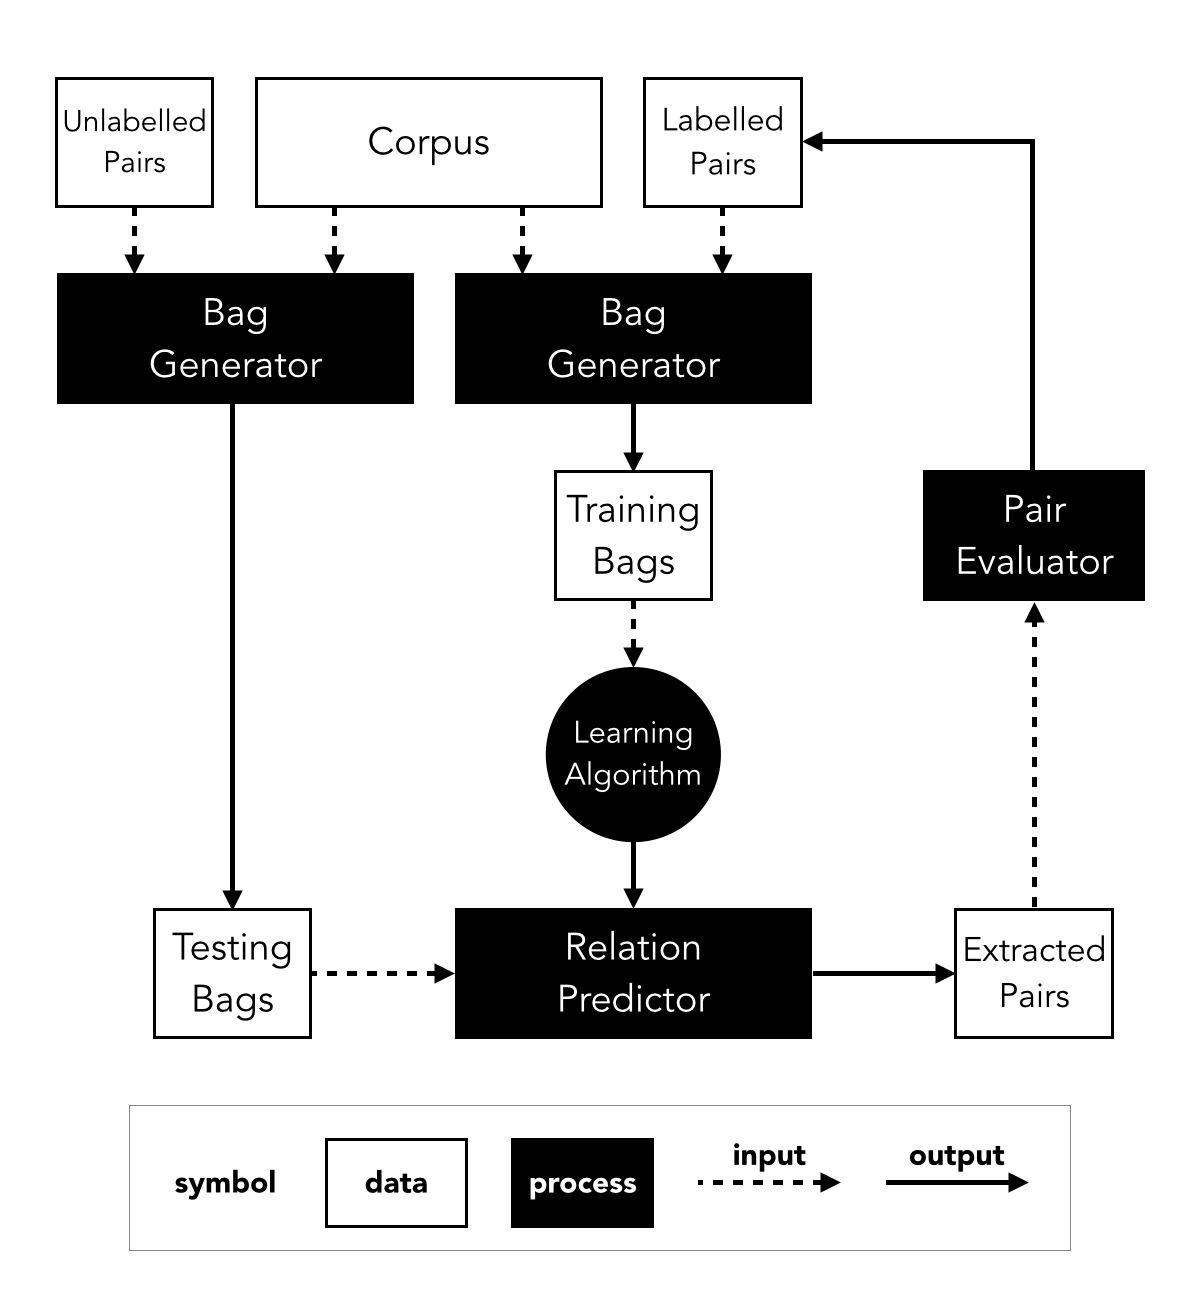
\includegraphics[width=1\textwidth]{framework.jpg}
\caption[Framework of the relational pair extraction system]{Framework of the relational pair extraction system}
\label{fig:framework}
\end{figure}

\subsection{Bag Generator}

The bag generator prepares training data and testing data for the relation predictor (Section \ref{method:RP}).
Each data is a bag, which collects sentences from a corpus and corresponds to an entity pair.
For example, a bag of the pair (``\textbf{Taipei}'', ``\textbf{Taiwan}'') consists of sentences mentioning ``\textbf{Taipei}'' and ``\textbf{Taiwan}'', such as ``\textbf{Taipei} is the capital of \textbf{Taiwan}'', ``\textbf{Taipei} is the political center of \textbf{Taiwan}''.
\par
In Figure \ref{fig:framework}, training bags are generated from labelled pairs and testing bags are generated from unlabelled pairs.
A labelled pair $(r, e_i, e_j)$ corresponds to a labelled bag $(y,b)$; an unlabelled data $(e_i,e_j)$ corresponds to an unlabelled bag $b$.
The bag generator aims at mapping pairs to bags.
If the pairs are labelled, the label will be brought to the bag.
\par
In this work, given a corpus $C$ and a labelled pair set, also known as seed set $S_r=\{(r,e_i,e_j)\}$, a training bag set $B_{train}$ is generated.
For each $(y,b)\in B_{train}$, $b$ is a bag of feature vectors and $y\in R$ refers to the label of this bag.
The details of feature vector are described in Section \ref{sec:method_feature}.
\par
Another bag set $B_{test}=\{b\}$ is used for testing.
It is generated with a corpus $C$ and an unlabeled pair set $U=\{(e_i,e_j) \mid e_i,e_j\in E\}$.
The details of automatic labelling are explained in Section \ref{sec:method_label}.
\par
The input and output of a bag generator is defined as following:
\begin{itemize}
\item \textbf{Input}: a corpus $C$, a pair set $S$
\item \textbf{Output}: a bag set $B$
\end{itemize}

\subsection{Relation Predictor}
\label{method:RP}
The relation predictor is used for generating new pairs from the corpus as a standard machine learning process.
With training bag set $B_{train}$ and an algorithm $\mathcal{A}$, the predictor is created to predict the label of each bag $b_i\in B_{test}$.
\par
In this work, tha algorithm $\mathcal{A}$ is a multiple instance learning algorithm due to the restriction of the problem.
More details of the multiple instance learning process are described in Section \ref{sec:method_mil}.
\par
The input and output of the relation predictor is defined as following:
\begin{itemize}
\item \textbf{Input}: a training bag set $B_{train}$, a testing bag set $B_{test}$, a learning algorithm $\mathcal{A}$
\item \textbf{Output}: a set of new pairs $N$
\end{itemize}

\subsection{Pair Evaluator}
To iteratively learn new pairs from the corpus, we update the seed set for each iteration.
To avoid using the false positive pairs as seeds in the next iteration, the result should be evaluated by another mechanism.
Here we use human intelligence as the evaluator.
\par
Given the new pair set $N^{(t)}_r$ generated in the $t^{th}$ iteration, we ask human to evaluate the correctness and generate another set $S^{(t+1)}_r$, which is the seed set in the next iteration.
The details of this process are illustrated in Section \ref{sec:method_iterate}.
\par
The input and output of the pair evaluator is defined as following:
\begin{itemize}
\item \textbf{Input}: a set of candidate pairs $N^{(t)}_r$
\item \textbf{Output}: a set of confident pairs $S^{(t+1)}_r$
\end{itemize}

%========== 我是framework的分隔線啊>"< ==========%

\section{Features of Data}
\label{sec:method_feature}
When generating the training data, we transfer plain texts to features, including syntactic, semantic, and textual forms. 
Zhou(2005)\cite{guodong2005exploring} has addressed several NLP features for relation extraction, including bag of words, parse tree, entity type, and other features.
Consider the example as following:

\begin{itemize}
\item Sentence
    \begin{itemize}
    \item[] 想到台大學生在校門口為言論自由絕食靜坐
    \item[] (think of Students from National Taiwan University sitting before the school gate, having hunger strike and sit-in demonstration for freedom of speech)
    \end{itemize}
\item Entity pair
    \begin{itemize}
    \item[] 學生(student), 校門(school gate)
    \end{itemize}
\end{itemize}

The features used in this thesis are shown in Table \ref{tab:feature_list}.
The part-of-speech tag\cite{Sinica_corpus} of this example is illustrated in Table \ref{tab:pos_tag_example} and dependency tree structure\cite{chang_zh_dep} is represented as Figure \ref{fig:dep_tree_example}\cite{syntree}.

\begin{table}
\begin{center}
\begin{tabular}{| c | m{6cm} | m{6cm} |}
\hline
Feature name    &   Explaination    &   Example\\
\hline\hline
W\_1    &   the first entity    &   學生\\
\hline
W\_2    &   the second entity   &   校門\\
\hline
BW\_1 &   bag of words before the first entity    &   想到, 台大\\
\hline
BW\_2 & bag of words after the second entity  &   口, 為, 言論, 自由, 絕食, 靜坐\\
\hline
BW\_12    &   bag of words between the 2 entities    &   在\\
\hline
POS\_1   &   pos tags before the first entity &   D, VE, Nc\\
\hline
POS\_2   &   pos tags after the second entity    &   Ncd, P, Na, Na, VA, VA\\
\hline
POS\_12  &   pos tags between the 2 entities &   P\\
\hline
DEP\_12  &   dependency tree structure between the 2 entities    &   NN $\leftarrow$ NP $\leftarrow$ IP $\rightarrow$ VP $\rightarrow$ PP $\rightarrow$ LCP $\rightarrow$ NP $\rightarrow$ NN\\
\hline
ORDER   &   order of the object and location    &   object $\rightarrow$ location\\
\hline
\end{tabular}
\captionsetup{width=0.8\textwidth}
\caption[List of features]{List of features, with the example related to sentence ``想到台大學生在校門口為言論自由絕食靜坐'' and entity pair (``學生'', ``校門'')}
\label{tab:feature_list}
\end{center}
\end{table}

\begin{table}
\begin{center}
\begin{tabular}{|ccccccccccc|}
\hline
想到 & 台大 & \textbf{\color{red}{學生}} & 在 & \textbf{\color{red}{校門}} & 口 & 為 & 言論 & 自由 & 絕食 & 靜坐\\
\hline
VE & Nc & \textbf{\color{red}{Na}} & P & \textbf{\color{red}{Na}} & Ncd & P & Na & Na & VA & VA\\
\hline
\end{tabular}
\captionsetup{width=0.8\textwidth}
\caption[part-of-speech example]{part-of-speech example related to sentence ``想到台大學生在校門口為言論自由絕食靜坐'', the red words are entity pairs}
\label{tab:pos_tag_example}
\end{center}
\end{table}

\begin{figure}
\centering
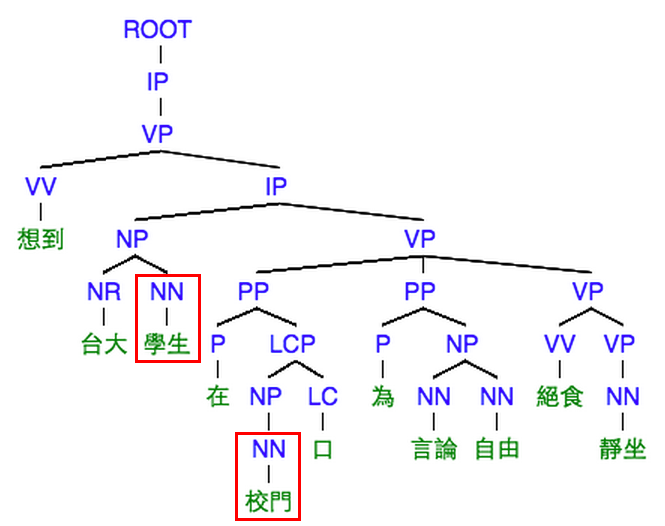
\includegraphics[width=0.8\textwidth]{dep_tree_example}
\captionsetup{width=0.8\textwidth}
\caption[dependency tree example]{dependency tree example related to sentence ``想到台大學生在校門口為言論自由絕食靜坐'', the words in red circles are entity pairs}
\label{fig:dep_tree_example}
\end{figure}

%========== 我是feature的分隔線Orz ==========%

\section{Assistant Labelling}
\label{sec:method_label}

Since the size of training bags used in this thesis is very large, it is difficult to label every data manually.
In this section, we propose a process to automatically label the training bags.
We follow the distant supervision assumption of relation extraction provided by Mintz(2009)\cite{mintz_distant}:

\newtheorem{theorem}{Assumption}
\begin{theorem}
\label{theo:ds}
If two entities participate in a relation, all sentences that mention these two entities express that relation.
\end{theorem}

With Assumption \ref{theo:ds}, we could match any seed $(r,e_i,e_j)$ to sentences mentioning $e_i$ and $e_j$, and assign the sentences with corresponding label $r$.
But this assumption is too strong because not all sentences containing $(e_i,e_j)$ express the relation $r$.
So Hoffmann(2011)\cite{hoffmann_knowledge} addressed a modified assumption by adapt the problem to a multiple instance learning problem.

\begin{theorem}
\label{theo:mil}
If two entities participate in a relation, at least one sentence that mentions these two entities might express that relation.
\end{theorem}

According to Assumption \ref{theo:mil}, given any seed $(r,e_i,e_j)$ and a bag of sentences mentioning $e_i$ and $e_j$, at least one sentences in the bag might express $r$.
Instead of describing a relation with a $sentence$, here we use a $bag$ to represent a relation.
The Assumption \ref{theo:mil} is midified as following:

\begin{theorem}
\label{theo:my}
If two entities participate in a relation, a bag of sentences that mention these two entities might express that relation.
\end{theorem}

Any entity pair $(r, e_i, e_j)$ in the seed set may correspond to a bag of sentences $b \subset C$, where each sentence $s \in b$ contains the 2 entity $e_i$ and $e_j$.
Then we decide the label $y$ for any $b$.
When at least one sentence in $b$ represents the relation $r$, $y=r$.
Otherwise, if the given relation $r$ does not shown in $b$, $y=null$.
The process of automatic labelling for an entity pair $(e_i, e_j)$ and corresponding set $b$ is displayed in Algorithm \ref{algo:auto_label}.

\begin{algorithm}
\begin{algorithmic}[1]
\renewcommand{\algorithmicrequire}{\textbf{Input:}}
\renewcommand{\algorithmicensure}{\textbf{Output:}}
    \REQUIRE a corpus $C={s}$, a seed set $S_r = \{(r,e_i,e_2)\ \mid r\in R;\; e_i,\,e_2\in E\}$
    \ENSURE a labelled bag set $B_{train} = \{(y,b)\}$
    \STATE initial a bag set $B$
    \FORALL{$(r,e_i,e_j) \in S_r$}
    \STATE generate a sentence set: $b_i=\{s \mid s\in C; e_j,\ e_k\ are\ words\ in\ s\}$
    \STATE assign the label for $b_i$: $y_i = r_i$
    \STATE add $(y_i,b_i)$ to $B$
    \ENDFOR
    \RETURN $B$
\end{algorithmic}
\caption[Process of automatic labelling training data]{Process of automatic labelling training data}
\label{algo:auto_label}
\end{algorithm}

%========== 哈囉我是Assistant Labelling的分隔線唷 ==========%

\section{Multiple Instance Learning}
\label{sec:method_mil}
Since we adapt the assumption of multiple instance learning to the problem, we choose the algorithm of multiple instance classifier as our core process in the system.

\subsection{Instance Space Learning}
\subsection{Bag Space Learning}
\subsection{Embedded Space Learning}

%========== 我是Multiple Instance Learning的分隔線zzzzz ==========%

\section{Iteratively Learning Process}
\label{sec:method_iterate}

%==========以下為暫存區==========%

\begin{comment}

\section{Framework}
The key process in this system is to build a \textbf{relation predictor} for deciding the relation of new pairs.
Before training this predictor, we have to transfer the sentences and seed from plain texts to training data by a \textbf{data processor}.

\subsection{Notation}
First, we define an entity set as $E=\{e_i | i \in \mathbb{N}\}$, and a relation set as $R=\{r_i | i \in \mathbb{N}\}$.
Each $e$ in $E$ represents a concept and $r$ in $R$ indicates a semantic relation used for linking 2 concepts.
Given an entity set, there is a corresponding corpus $S=\{s_i | i \in \mathbb{N}\}$, where each $s$ is a sentence constructed by $e$ in $E$.
And a seed contains an entity pair $p=(e_i, e_j), e_i, e_j \in E$ and a lebel $r$, indicating that $e_i$ and $e_j$ are semantically related by a relation $r \in R$. 
Thus, we define a seed set as $Seed=\{(r, p) | r \in R; p \in E \times E\}$.

\subsubsection{Data processor}
The data processor is used for transferring plain texts to training data, with assistance of entity pair seeds.
The plain texts are sentences in a corpus $S$, where $S=\{s_1, s_2, ..., s_N\}$.
Each $s$ in $S$ refers to a segmented sentence as a list of words, where $s=\{w_1, w_2, ..., w_K\}$.
And the entity pair seeds are in a seed pool $C$, where $C=\{c_1, c_2, ..., c_N\}$.
Each $c$ in $C$ contains an entity pair $p=(e_{front}, e_{back})$ and a label $r$ indicating whether the relation exists between $e_{front}$ and $e_{back}$, that is, $c=(r, p)$.

\begin{enumerate}
\item $Corpus$ is a set of sentences serves for generating training data and new knowledge. 
\item $Candidate\ seeds$ are entity pairs correspond to a specific relation. They could refer to the initial knowledge or extracted new knowledge.
\item $Confident\ seeds$ are reliable seeds selecting from candidate seeds. In this thesis, they are selected manually.
\item $Training\ data$ is the data used for training a classifier for each iteration.
\item $Testing\ data$ is the data used for testing the new classifier for each iteration.
\end{enumerate}

\subsubsection{Relation predictor}
The relation predictor is used for predicting whether a pair contains the relation $AtLocation$.
Each training data is a bag, containing several data.
We define a training bag set as $B_{train}$, where $B_{train}=\{(y_1,b_1), (y_2,b_2), ..., (y_N,b_N)\}$.
In each $(y,b)$ in $B$, $y$ indicates the label of a bag, and $b$ is a list of vectors representing the features of bag.
Another bag set $B_{test}$ is used for testing, where $B_{test}=\{b_1, b_2, ..., b_Z\}$.
The format of $B_{test}$ is viewed as $B_{train}$ without labels.
For any bag in $B_{train}$ or $B_{test}$, there is a corresponding entity pair $(e_{front}, e_{back})$.
After the relation predictor predicts the data in $B_{test}$, some results is shown as the form of pair list, where $P=\{p_1, p_2, ..., p_X\}$.

\begin{enumerate}
\item $Pair\ list$ is a list of entity pairs. Each entity pairs contains 2 entity with some kind of relation.
\item $Classifier$ is used for predicting whether a new data has the specific relation. It is created by a supervised learning algorithm.
\item $Maxinum\ iteration$ refer to a predifined interger. When the number of training iteration reachs this given number, the system will stop training.
\end{enumerate}

\subsection{Problem Definition}
In the problem of relational pair extraction, we define the input and output as following:
\begin{itemize}
\item \textbf{Input}: a seed pool $C$, a corpus $S$, maximal number of iteration $Max$
\item \textbf{Output}: a set of new pairs $P$
\end{itemize}

\subsubsection{Data processor}
For data processor, we define the input and output as following:
\begin{itemize}
\item \textbf{Input}: a seed pool $C$, a corpus $S$
\item \textbf{Output}: a set of training data $B_{train}$, a set of testing data $B_{test}$
\end{itemize}

\subsubsection{Relation predictor}
For relation predictor, we define the input and output as following:
\begin{itemize}
\item \textbf{Input}: a set of training data $B_{train}$, a set of testing data $B_{test}$
\item \textbf{Output}: a set of new pairs $P$
\end{itemize}

\paragraph{Select confident seeds}
The process of selecting confident seeds is required since the exterior source may not be reliable.
If the seeds are from a knowledge base generated by crowd sourcing, the quality of data may not be guaranteed.
In this case, we use the selected seeds instead of all.
Human intelligence is considered as reliable classifier to decide whether 2 concepts are linked by a given relation.
To avoid wasting manual power, we only consider the seeds correlated to the corpus.

\paragraph{Generate data}
To go through a supervised learning learning process, training data are used for training and testing data are used for evaluating.
In distant supervision, all data are not labelled initially.
With the assistance of exterior knowledge base, the data are given labels and transferred from plain texts to vectors.
The details of automatic labelling are explained in Section \ref{sec:method_label}, and the features used in this thesis are described in Section\ref{sec:method_feature}. 

\paragraph{Train a classifier}
With training data and testing data, we consider different supervised classication methods as the training algorithms.
Since the system is under the skeleton of multiple instance learning (MIL), the algorithms are adapted to MIL setting.
More details about the learning process are demonstrated in Section \ref{sec:method_mil}.

\paragraph{Predict candidate seeds}
The initial candidate seeds are from existing knowledge base.
After the first iteration of training, a predictor would be created for classifying testing data as positive or negative.
Those data decided as positive could be used as seeds for retraining in the next iteration.
Since the predictor is not perfect enough, the candidate seeds could not be used directly.
Instead, as the first step, candidate seeds should be manually filtered as confident seeds.

\end{comment}

\chapter{Experiment and Result}
This chapter shows the experiment for Chinese relational pair extraction.
First, the data source and data generating process will be explained.
Then the experimentl setting will be presented in the second section.
In the last 2 sections, the result for testing the proposed framework with given data will be discussed.

\section{Dataset}
Distant supervision learning, which is an semi-supervised framework, uses small size of labelled data and huge size of unlabelled data for training.
In relation extraction work, the labelled data are usually from an existing dataset and the unlabelled data are from a huge corpus containing many sentences, such as news corpus or Wikipedia.
In this thesis, we use Chinese entities pairs from ConceptNet as labeled data and sentences in Taiwan Sinica Corpus as unlabeled data.

\subsection{ConceptNet}
ConceptNet is developed by MIT Media Lab\cite{ConceptNet5}, containing only English data at beginning.
It is a graphical structure, with node representing $concept$, and link representing $relation$, describing a commonsense knowledge base.
A commonsense fact, formulated as two concepts and one relation bwtween them, is called $assertion$, which is stored as 2 nodes ($concepts$) and 1 link ($relation$) in the ConceptNet graph.
The knowledge in ConceptNet is originally provided by human as crowesourcing.
Afterwards, the authors imported knowledge from other datasets such as WordNet, Wikipedia, Wikitionary, DBPedia, and other sources.
From ConceptNet 3, by collaborating with universities from different countries, ConceptNet absorbed data from other languages, becoming a multilingual commonsense dataset.
Chinese assertions are collected from an online pet game, by feeding the pets new knowledge.
\par
Before ConceptNet 4, the relations of ConceptNet is predefined.
When collecting knowledge in Chinese, only 15 relations are considered (shown in Table \ref{tab:relation_list}).
The relation $AtLocation$ represents the relationship between an object and a location. For example, $AtLocation(Taipei, Taiwen)$ indicates that ``Taipei is located in Taiwan''.
\par
Each assertion is regarded as labelled data when training a distant supervision model.
The experiment uses Chinese assertions related to the relation $AtLocation$.
Since Chinese assertions in ConceptNet are generated from online users, the reliability is not guaranteed.
Among all 32816 assertions, only about $37\%$ of data are valid for training.
The examples of seeds from ConceptNet are shown in Table \ref{tab:AtLocation_seed}.

\begin{table}[t]
\begin{center}
\begin{tabular}{lcc}
\hline
Relation Name   & Number of Assertions\\  
\hline
AtLocation  & 32816\\
CausesDesire & 19408\\
HasProperty & 6822\\
NotDesires & 23930\\
UsedFor & 13548\\
Causes & 77336\\
HasSubevent & 40655\\
PartOf & 6159\\
Desires & 21772\\
IsA & 16094\\
HasFirstSubevent & 12046\\
MadeOf & 16357\\
CapableOf & 27444\\
SymbolOf & 4736\\
MotivatedByGoal &56636\\
\hline
\end{tabular}
\caption[List of relations corresponding to Chinese knowledge in ConceptNet]{\small List of relations corresponding to Chinese knowledge in ConceptNet}
\label{tab:relation_list}
\end{center}
\end{table}

\begin{table}[t]
\begin{center}
\begin{tabular}{| c | l | l |}
\hline
label  &   entity (object)   &    entity (location)\\
\hline
O   &   教授(professor)   &   研究所 (graduate school)\\
O   &   員工 (staff)   &   公司 (company)\\
O   &   人民 (people)   &   台灣 (Taiwan)\\
O   &   學生 (student)   &   學校 (school)\\
O   &   病人 (patient)   &   醫院 (hospital)\\
O   &   鯉魚 (carp)   &   池塘 (pond)\\
X   &   美國 (USA)   &   亞洲 (Asia)\\
X   &   程式 (program)   &   電腦 (computer)\\
X   &   太陽 (sun)   &   夏天 (summer)\\
X   &   觀眾 (audience)   &   電視 (television)\\
\hline
\end{tabular}
\caption[Example of positive and negative entity pairs of Chineses knowledge in ConceptNet]{\small Example of positive and negative entity pairs of Chineses knowledge in ConceptNet}
\label{tab:AtLocation_seed}
\end{center}
\end{table}

%==========我是ConceptNet的分隔線==========%
\subsection{Sinica Corpus}
The full name of Sinica Corpus\cite{Sinica_corpus} is ``Academia Sinica Balanced Corpus of Modern Chinese'', developed from 1994.
This corpus contains articles from 1981 to 2007, spread in different fields including philosophy, science, society, art, life, and literature.
The source of articles is also diverse, including news, book, textbook, magazine, and so on, which shows the corpus contains different styles of articles.
Each article is stored as sentences by segmenting the article with comma, period, semicolon, question mark and exclamation mark.
In Chinese articles, the usage of comma is slightly different from English.
Sometimes, the sentence before the comma and after the comma can be independent in grammar while they may be dependent in meaning.
The corpus is separated as about 6 hundred thousand sentences and each sentence is segmented as words.
Each word is annotated with a part-of-speech tag.
Since the articles of Sinica Corpus are cross many years, the phrasing may be slightly diferent to the wording nowadays.
The wording is more conscientious and careful because the sources are formal media.
The example of sentences are shown on Table \ref{tab:sa_example}
\par
The experiment uses the sentences in Sinica Corpus as unlabelled data.
Each sentences are regarded as a list of words and each 2 words in the sentence may convey one or no relation.
The method for generating training data from sentences is described in Section \ref{sec:method_label} on page \pageref{sec:method_label}.

\begin{table}[t]
\begin{center}
\begin{tabular}{| m{10cm} | m{6cm} |}
\hline
Sentence   &   Translation\\
\hline
{\small 民族學(Na) 研究所(Nc) 應(D) 主持(VC) 之(DE) 「(PARENTHESISCATEGORY) 台灣(Nc) 與(Caa) 東南亞(Nc) 土著(Na) 文化(Na) 與(Caa) 血緣(Na) 關係(Na) 」(PARENTHESISCATEGORY) 主題(Na) 研究(Nv) 計劃(Na) 之(DE) 需要(Na) ,(COMMACATEGORY)}  &   {According to the need for hosting the research project ``aboriginal culture and blood relationship bwtween Taiwan and Southeast Asia'', Institute of Ethnology ...}\\
\hline
{\small 邀請(VC) 蘇聯(Nc) 國家(Na) 科學院(Nc) 世界(Nc) 文學(Na) 研究所(Nc) 研究員(Na) Boris(FW) Parnickel(FW) 教授(Na) 於(P) 六月(Nd) 十九日(Nd) 至(P) 廿六日(Nd) 來訪(VA) ,(COMMACATEGORY)}  &   {... invited the researcher, Professor Boris Parnickel, who comes from Institute of World Literature of Russian Academy of Sciences, to visit from 19th to 26th June.}\\
\hline
{\small Boris(FW) 教授(Na) 之(DE) 專長(Na) 為(VG) 東南(Ncd) ((PARENTHESISCATEGORY) 特別(VH) 是(SHI) 馬來亞(Nc) 及(Caa) 印尼(Nc) )(PARENTHESISCATEGORY) 的(DE) 神話(Na) 傳說(Na) 及(Caa) 民俗(Na) ,(COMMACATEGORY)}   &   {Professor Boris specializes in the legend and folklore in Southeast Asia, especially in Malaysia and Indonesia, ...}\\
\hline
{\small 在(P) 此(Nep) 一(Neu) 領域(Na) 已(D) 有(V\_2) 傑出(VH) 之(DE) 研究(Nv) 成果(Na) 。(PERIODCATEGORY)}   &   {... having excellent achievements in this area.}\\
\hline
\end{tabular}
\caption[Example of sentences in Sinica Corpus]{Example of sentences in Sinica Corpus}
\label{tab:sa_example}
\end{center}
\end{table}

%==========我是平衡語料庫分隔線==========%
\subsection{UDN News Dataset}
\par
UDN.com is a news website in Taiwan, reporting various types of online news.
Different from Sinica Corpus, articles in UDN news are less formal, including many novel terms.
Sentences in UDN news are used as unlabelled data.
Articles are segmented to sentences by a period stop, which may conserve complete meaning in the sentence.
The articles are raw texts without any label or processing.
Before training, these sentences have to be segmented to words, labelled with part-of-speech tag, and other grammatically parsed with external NLP tools.
\par
There are two sets of UDN data collected for experiment.
One is recent news on the real time news column (from February to May 2015), and another is historical news in the past 10 years, including 3 different columns.
The difference of these 2 dataset is the size and age of news.

\section{Experiment setting}

\subsection{Experiment 1: Feature selection}
\subsection{Experiment 2: MIL Algorithm selection}
\subsection{Experiment 3: Iteration}
\subsection{Experiment 4: Multiple Relations}

\section{Evaluation}
We use $Accuracy$ for evaluating the result of cross validation:

\begin{equation}
Accuracy = \frac{\abs{accuate\ testing\ data}}{\abs{total\ testing\ data}}
\label{eq:accuracy}
\end{equation}

\section{Result and Discussion}

\chapter{Application}

%\section{Assistant for ConceptNet}
%\section{Article Analysis}

\chapter{Conclusion}


\appendix

\backmatter

\addcontentsline{toc}{chapter}{\bibname}
\bibliographystyle{abbrv}

% Your bibliography goes here
\bibliography{thesis}

\end{document}
